In this section we introduced  a walking task to deal with the drift generated on the yaw angle of the robot when walking while holding the fire hose, as explained in the previous section.
%
Then, simulation results are shown to confirm the validity of the proposed walking task.



To cope with the drift in the walking direction explained in the previous section, we introduced a walking task $\mathbf{e}_w$ which is defined as:
%
\begin{equation}
\mathbf{e}_w = \mathbf{x} - \mathbf{x}_d \; ,
\label{ewalk}
\end{equation}
%
where vector $\mathbf{x} = [x_c \; y_c \; \phi_c]^T$ includes the robot's chest $X$ and $Y$ direction position and its yaw orientation angle $\phi$. Similarly, the desired position and yaw angle is represented by $\mathbf{x}_d$.
%
Therefore, the desired reference velocity for walking $\mathbf{v}^{\text{ref}}$ is obtained as:
%
\begin{equation}
\mathbf{v}^{\text{ref}} = -\lambda \mathbf{e}_{w} - \mathbf{\Lambda} \int \mathbf{e}_{w}(t)  \; \mathrm{d}t \; ,
\label{velwalk}
\end{equation}
%
where $\lambda$ is an adaptive gain and the matrix $\mathbf{\Lambda}$ is a diagonal matrix of adaptive gains. 
%
The obtained reference velocity is used as an input to the walking pattern generator that will calculate the footsteps of the robot in real time, and also as an input to the impedance controller that will compute the desired pulling force according to the robot's reference velocity.
%
Fig.~\ref{sim_graph} shows the simulation results for a walking task with $\mathbf{x}_d = [4.0 \; 0.0 \; 0.0]^T$ when the robot starting position is $\mathbf{x}_i = [0.0 \; 0.0 \; 0.0]^T$.
%
A maximal velocity of $0.10$ and $0.15$ m/step for the $X$ and $Y$ directions, respectively, and $5$ deg/step are set to the walking task.
%
%
\begin{figure}[t]
 \centering
 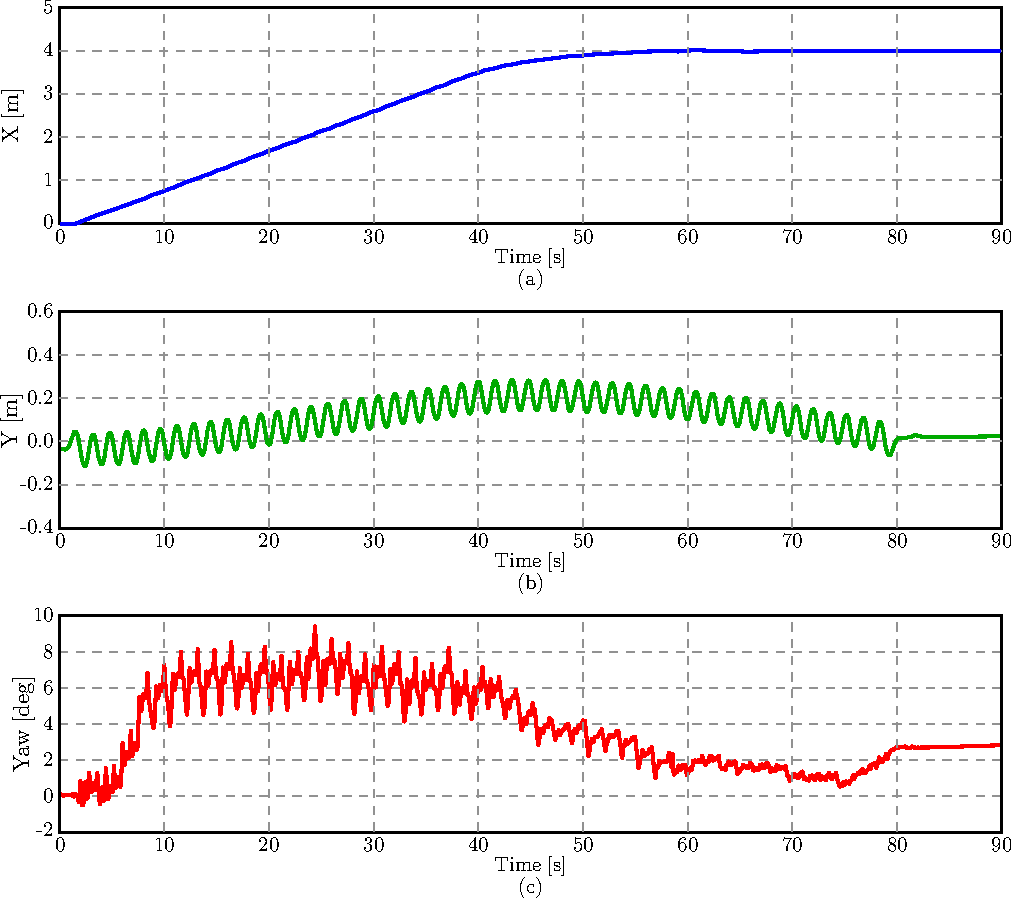
\includegraphics[height=0.40\textwidth]{./figures/sim_pos.pdf}
 \vspace{-3mm}
 \caption{Robot's waist trajectory in simulation. In (a) position in $X$ direction, in (b) position in $Y$ direction and in (c) yaw angle.}
 \label{sim_graph}
% \vspace{-5mm}
\end{figure}
%
%
It can be seen that the robot reaches the desired position within $80$ seconds and also that the walking task is able to correct the drift generated by the hose.
